\chapter{Bullseye: A parallel targeted facet imager}
\section{Design objectives}
The primary design objectives of this work is to build a scalable parallel facet-based imager. A full deconvolution pipeline is currently out of scope, instead 
the focus is on accelerating the gridding step, since this step will be called on multiple times in a major-minor cycle deconvolution pipeline as discussed in 
chapter \ref{chapter_synthesis}. To this end we will focus on comparing performance between parallel CPU-based resampling and a GPU approach.
\section{Architecture}
We've decided to split up the our implementation into two major components:
\begin{enumerate}
 \item A front-end program dealing with the logic of reading in measurement data, dealing with user options, overall program flow and image finalization.
 \item A set of back-end libraries that implement a common interface and house the resampling and transformation routines. The resampling routines include options to resample multiple
 correlations and enable faceting and w-projection logic.
\end{enumerate}

The architecture above allows us to easily swap out one set of resampling routines for another and to compare between CPU and GPU-based implementations. Figure~\ref{fig_arch} shows
the major components of our imager, along with several major dependencies. 
\begin{figure}[h]
  \begin{mdframed}
    \centering
    \begin{subfigure}[b]{0.66\textwidth}
      \centering
      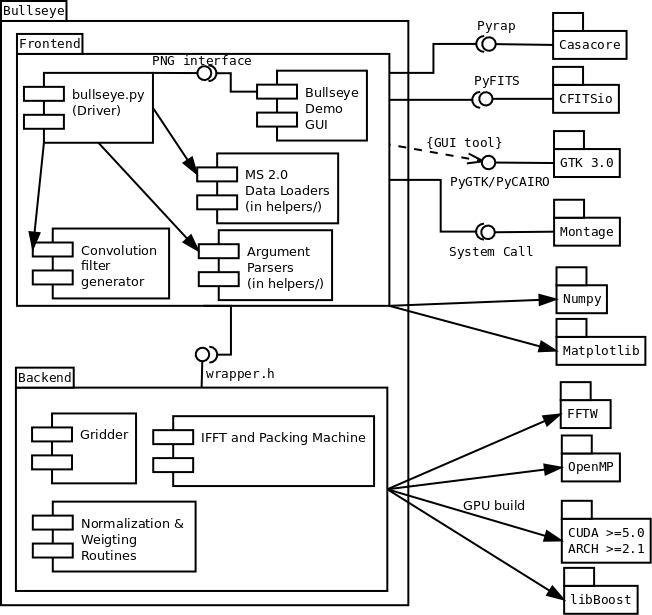
\includegraphics[width=\textwidth]{images/bullseye_arch.png}
      \caption{}
    \end{subfigure}  
    \caption[Bullseye Architecture]{The front end of the solution contains a commandline utility that has very similar options to that provided in other imagers, such as lwimager.
    Included with it are modules required to generate the w-projection convolution functions and a prototype graphical interface illustrating targeted faceting. The backend consists
    of the resampling routines along with routines to do fourier shifting, inversion and normalization on a set of facets that may each contain multiple spectral images.}
    \label{fig_arch}
  \end{mdframed}
\end{figure}
\section{Normal workflow}
During imaging the user will supply a set of facet centre coordinates, number of facets in l and m or both, along with a measurements database and outputs a set of facet images that can optionally
be recombined with the astronomical mosaicking package, Montage.
\section{Input/Output formats}
\subsection{NRAO Measurement Set 2.0}
\subsection{The Flexible Image Transport System}
\section{Targeted faceting and image mosaicking options}
\section{Continuum imaging vs. spectral line imaging}
\section{Work distribution strategies considered}
\subsection{CPU}
\subsection{GPU}